% Physical picture of grain-boundary oxidation with and without prior irradiation.
% Six panels, 2 x 3, each ~5.6 x 5.0 cm; styled to match framework_a-d.
\documentclass[12pt,border=2pt,tikz]{standalone}

\usepackage{amsmath}
\usepackage{mhchem}

\usetikzlibrary{arrows.meta}

\definecolor{cOx}{RGB}{250,224,80}      % oxide
\definecolor{cOxLow}{RGB}{222,160,40}   % Cr-poor oxide
\definecolor{cMetal}{RGB}{214,214,211}
\definecolor{cWater}{RGB}{158,206,232}
\definecolor{cEdge}{RGB}{40,40,44}
\definecolor{cAcc}{RGB}{20,72,124}      % oxygen
\definecolor{cRIS}{RGB}{24,104,66}      % segregation
\definecolor{cRISBg}{RGB}{225,240,232}  % segregated zone
\definecolor{cGB}{RGB}{96,42,140}
\definecolor{cRed}{RGB}{158,54,42}      % metal leaving through the oxide
\definecolor{cCr}{RGB}{17,119,51}
\definecolor{cNi}{RGB}{0,90,181}
\definecolor{cSi}{RGB}{214,96,20}
\definecolor{cDef}{RGB}{110,110,112}    % point defects

\begin{document}
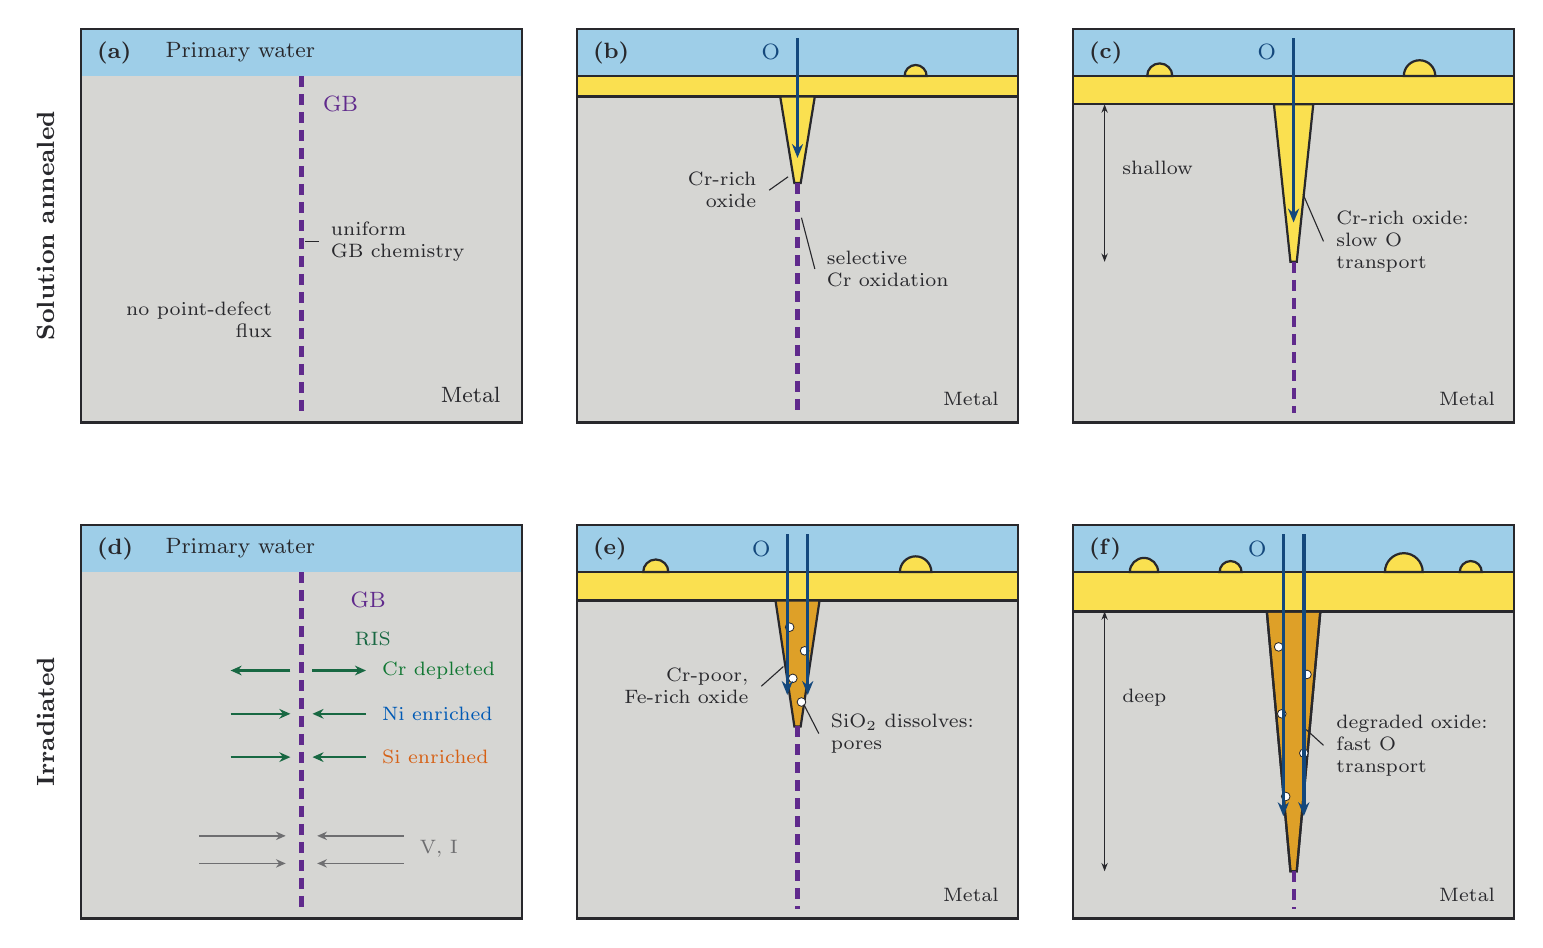
\begin{tikzpicture}[
  x=1cm,y=1cm, font=\footnotesize, color=cEdge,
  eg/.style   ={draw=cEdge, line width=0.8pt},
  flux/.style ={-{Stealth[length=5pt,width=4pt]},   line width=1.25pt, draw=cAcc},
  ris/.style  ={-{Stealth[length=4pt,width=3.5pt]}, line width=0.9pt,  draw=cRIS},
  leave/.style={-{Stealth[length=4pt,width=3.5pt]}, line width=0.9pt,  draw=cRed},
  def/.style  ={-{Stealth[length=3.5pt,width=3pt]}, line width=0.6pt,  draw=cDef},
  lead/.style ={draw=cEdge, line width=0.4pt},
  key/.style  ={font=\scriptsize, color=cEdge},
  gbline/.style={draw=cGB, line width=1.5pt, dash pattern=on 4pt off 2.5pt},
]

\def\W{5.60}\def\H{5.00}\def\yWb{4.40}   % panel size; water occupies y > \yWb
\def\xc{2.80}                            % grain-boundary plane

% ----- panel background: #1 = surface-oxide thickness ---------------------
\newcommand{\base}[1]{%
  \fill[cWater] (0,\yWb) rectangle (\W,\H);
  \fill[cMetal] (0,0)    rectangle (\W,\yWb);
  \ifdim #1pt>0pt \fill[cOx,eg] (0,\yWb-#1) rectangle (\W,\yWb);\fi
  \draw[eg] (0,0) rectangle (\W,\H);
}
% ----- segregated zone along the boundary: #1 = top y -------------------
\newcommand{\risband}[1]{\fill[cRISBg] (\xc-0.42,0.02) rectangle (\xc+0.42,#1);}
% ----- intergranular oxide wedge: #1 top y, #2 depth, #3 half-width, #4 fill
\newcommand{\wedgeox}[4]{%
  \fill[#4,eg] (\xc-#3,#1) -- (\xc+#3,#1) -- (\xc+0.04,#1-#2) -- (\xc-0.04,#1-#2) -- cycle;}
% ----- outer oxide particle on the surface: #1 x, #2 radius --------------
\newcommand{\particle}[2]{\fill[cOx,eg] (#1-#2,\yWb) arc (180:0:#2) -- cycle;}
% ----- pore -------------------------------------------------------------
\newcommand{\pore}[2]{\fill[white,draw=cEdge,line width=0.3pt] (#1,#2) circle (0.055);}

% =========================================================================
% Row labels and column titles
% =========================================================================
\node[rotate=90,font=\small\bfseries] at (-0.45,6.30+\H/2) {Solution annealed};
\node[rotate=90,font=\small\bfseries] at (-0.45,\H/2)      {Irradiated};

% =========================================================================
% (a) solution annealed, before exposure
% =========================================================================
\begin{scope}[shift={(0,6.30)}]
  \base{0}
  \draw[gbline] (\xc,\yWb) -- (\xc,0.12);
  \node[anchor=north west,font=\footnotesize\bfseries] at (0.08,\H-0.04) {(a)};
  \node[anchor=west] at (0.95,\yWb+0.30) {Primary water};
  \node[anchor=east] at (\W-0.15,0.35) {Metal};
  \node[anchor=west,cGB] at (\xc+0.15,\yWb-0.35) {GB};
  \node[key,anchor=west,align=left] at (\xc+0.25,2.30)
        {uniform\\ GB chemistry};
  \draw[lead] (\xc+0.22,2.30) -- (\xc+0.04,2.30);
  \node[key,anchor=east,align=right] at (\xc-0.25,1.30)
        {no point-defect\\ flux};
\end{scope}

% =========================================================================
% (b) solution annealed, early exposure
% =========================================================================
\begin{scope}[shift={(6.30,6.30)}]
  \base{0.26}
  \def\ys{4.14}
  \wedgeox{\ys}{1.10}{0.22}{cOx}
  \draw[gbline] (\xc,\ys-1.10) -- (\xc,0.12);
  \particle{4.30}{0.14}
  \node[anchor=north west,font=\footnotesize\bfseries] at (0.08,\H-0.04) {(b)};
  % oxygen in
  \draw[flux] (\xc,\H-0.12) -- (\xc,\ys-0.78);
  \node[anchor=east,cAcc] at (\xc-0.10,\yWb+0.30) {O};
  % Cr-rich oxide
  \node[key,anchor=east,align=right] at (\xc-0.40,2.95) {Cr-rich\\ oxide};
  \draw[lead] (\xc-0.36,2.95) -- (\xc-0.12,3.12);
  \node[key,anchor=west,align=left] at (\xc+0.25,1.95) {selective\\ Cr oxidation};
  \draw[lead] (\xc+0.22,1.95) -- (\xc+0.05,2.60);
  \node[anchor=east,font=\scriptsize] at (\W-0.12,0.30) {Metal};
\end{scope}

% =========================================================================
% (c) solution annealed, extended exposure
% =========================================================================
\begin{scope}[shift={(12.60,6.30)}]
  \base{0.36}
  \def\ys{4.04}
  \wedgeox{\ys}{2.00}{0.25}{cOx}
  \draw[gbline] (\xc,\ys-2.00) -- (\xc,0.12);
  \particle{1.10}{0.16}\particle{4.40}{0.20}
  \node[anchor=north west,font=\footnotesize\bfseries] at (0.08,\H-0.04) {(c)};
  \draw[flux] (\xc,\H-0.12) -- (\xc,\ys-1.50);
  \node[anchor=east,cAcc] at (\xc-0.10,\yWb+0.30) {O};
  % protective oxide
  \node[key,anchor=west,align=left] at (\xc+0.42,2.30) {Cr-rich oxide:\\ slow O\\ transport};
  \draw[lead] (\xc+0.38,2.30) -- (\xc+0.12,2.90);
  % depth
  \draw[{Stealth[length=3pt]}-{Stealth[length=3pt]},line width=0.5pt]
        (0.40,\ys) -- (0.40,\ys-2.00);
  \node[key,anchor=west] at (0.50,\ys-0.80) {shallow};
  \node[anchor=east,font=\scriptsize] at (\W-0.12,0.30) {Metal};
\end{scope}

% =========================================================================
% (d) irradiated, before exposure
% =========================================================================
\begin{scope}[shift={(0,0)}]
  \base{0}
  \draw[gbline] (\xc,\yWb) -- (\xc,0.12);
  \node[anchor=north west,font=\footnotesize\bfseries] at (0.08,\H-0.04) {(d)};
  \node[anchor=west] at (0.95,\yWb+0.30) {Primary water};
  \node[anchor=west,cGB] at (\xc+0.50,\yWb-0.35) {GB};
  % segregation: Cr away, Ni and Si towards the boundary
  \node[anchor=west,cRIS,font=\scriptsize] at (\xc+0.55,3.55) {RIS};
  \draw[ris] (\xc+0.14,3.15) -- (\xc+0.82,3.15);
  \draw[ris] (\xc-0.14,3.15) -- (\xc-0.90,3.15);
  \node[anchor=west,cCr,font=\scriptsize] at (\xc+0.90,3.15) {Cr depleted};
  \draw[ris] (\xc+0.82,2.60) -- (\xc+0.14,2.60);
  \draw[ris] (\xc-0.90,2.60) -- (\xc-0.14,2.60);
  \node[anchor=west,cNi,font=\scriptsize] at (\xc+0.90,2.60) {Ni enriched};
  \draw[ris] (\xc+0.82,2.05) -- (\xc+0.14,2.05);
  \draw[ris] (\xc-0.90,2.05) -- (\xc-0.14,2.05);
  \node[anchor=west,cSi,font=\scriptsize] at (\xc+0.90,2.05) {Si enriched};
  % point defects to the boundary
  \draw[def] (\xc+1.30,1.05) -- (\xc+0.20,1.05);
  \draw[def] (\xc-1.30,1.05) -- (\xc-0.20,1.05);
  \draw[def] (\xc+1.30,0.70) -- (\xc+0.20,0.70);
  \draw[def] (\xc-1.30,0.70) -- (\xc-0.20,0.70);
  \node[anchor=west,cDef,font=\scriptsize] at (\xc+1.38,0.88) {V, I};
\end{scope}

% =========================================================================
% (e) irradiated, early exposure
% =========================================================================
\begin{scope}[shift={(6.30,0)}]
  \base{0.36}
  \def\ys{4.04}
  \wedgeox{\ys}{1.60}{0.28}{cOxLow}
  \draw[gbline] (\xc,\ys-1.60) -- (\xc,0.12);
  \particle{1.00}{0.16}\particle{4.30}{0.20}
  \pore{\xc-0.10}{3.70}\pore{\xc+0.09}{3.40}\pore{\xc-0.06}{3.05}\pore{\xc+0.05}{2.75}
  \node[anchor=north west,font=\footnotesize\bfseries] at (0.08,\H-0.04) {(e)};
  % more oxygen in
  \draw[flux] (\xc-0.13,\H-0.12) -- (\xc-0.13,\ys-1.20);
  \draw[flux] (\xc+0.13,\H-0.12) -- (\xc+0.13,\ys-1.20);
  \node[anchor=east,cAcc] at (\xc-0.22,\yWb+0.30) {O};
  % labels
  \node[key,anchor=east,align=right] at (\xc-0.50,2.95) {Cr-poor,\\ Fe-rich oxide};
  \draw[lead] (\xc-0.46,2.95) -- (\xc-0.18,3.20);
  \node[key,anchor=west,align=left] at (\xc+0.30,2.35) {\ce{SiO2} dissolves:\\ pores};
  \draw[lead] (\xc+0.27,2.35) -- (\xc+0.08,2.72);
  \node[anchor=east,font=\scriptsize] at (\W-0.12,0.30) {Metal};
\end{scope}

% =========================================================================
% (f) irradiated, extended exposure
% =========================================================================
\begin{scope}[shift={(12.60,0)}]
  \base{0.50}
  \def\ys{3.90}
  \wedgeox{\ys}{3.30}{0.34}{cOxLow}
  \draw[eg] (\xc-0.34,\ys) -- (\xc+0.34,\ys) -- (\xc+0.04,\ys-3.30) -- (\xc-0.04,\ys-3.30) -- cycle;
  \draw[gbline] (\xc,\ys-3.30) -- (\xc,0.12);
  \particle{0.90}{0.18}\particle{2.00}{0.14}\particle{4.20}{0.24}\particle{5.05}{0.14}
  \pore{\xc-0.19}{3.45}\pore{\xc+0.17}{3.10}\pore{\xc-0.15}{2.60}\pore{\xc+0.13}{2.10}\pore{\xc-0.10}{1.55}
  \node[anchor=north west,font=\footnotesize\bfseries] at (0.08,\H-0.04) {(f)};
  \draw[flux] (\xc-0.13,\H-0.12) -- (\xc-0.13,\ys-2.60);
  \draw[flux] (\xc+0.13,\H-0.12) -- (\xc+0.13,\ys-2.60);
  \node[anchor=east,cAcc] at (\xc-0.22,\yWb+0.30) {O};
  % labels
  \node[key,anchor=west,align=left] at (\xc+0.42,2.20) {degraded oxide:\\ fast O\\ transport};
  \draw[lead] (\xc+0.38,2.20) -- (\xc+0.16,2.40);
  % depth
  \draw[{Stealth[length=3pt]}-{Stealth[length=3pt]},line width=0.5pt]
        (0.40,\ys) -- (0.40,\ys-3.30);
  \node[key,anchor=west] at (0.50,\ys-1.10) {deep};
  \node[anchor=east,font=\scriptsize] at (\W-0.12,0.30) {Metal};
\end{scope}

\end{tikzpicture}
\end{document}
